\documentclass[screen, authorversion, nonacm, sigconf]{acmart}

\usepackage[linesnumbered,commentsnumbered,ruled]{algorithm2e}
\usepackage{graphicx}
\usepackage{booktabs}

\begin{document}

\title{Exploring the Impact of Decision Tree Depth}

\author{Alic Szecsei}
\affiliation{University of Iowa}
\email{alic-szecsei@uiowa.edu}

\author{Diego Castaneda}
\affiliation{University of Iowa}
\email{diego-castaneda@uiowa.edu}

\author{Willem DeJong}
\affiliation{University of Iowa}
\email{willem-dejong@uiowa.edu}

\begin{abstract}
  Lobortis scelerisque fermentum dui faucibus in ornare quam viverra orci sagittis eu volutpat odio facilisis mauris sit amet massa vitae tortor condimentum lacinia quis vel eros donec ac odio tempor orci dapibus ultrices in iaculis nunc sed augue lacus viverra vitae congue eu consequat ac felis donec et odio pellentesque diam volutpat commodo sed egestas egestas fringilla phasellus faucibus scelerisque eleifend donec pretium vulputate sapien nec sagittis aliquam malesuada bibendum arcu vitae elementum curabitur vitae nunc sed velit dignissim sodales ut eu sem integer vitae justo eget magna fermentum iaculis eu non diam phasellus vestibulum lorem sed risus ultricies tristique nulla aliquet enim tortor at auctor urna nunc id cursus metus aliquam eleifend mi in nulla posuere sollicitudin aliquam ultrices sagittis orci a scelerisque purus semper eget duis at tellus at urna condimentum mattis pellentesque id nibh tortor id aliquet lectus proin nibh nisl condimentum id venenatis a condimentum vitae sapien pellentesque habitant morbi tristique senectus et netus et malesuada fames ac turpis egestas sed tempus urna et pharetra pharetra massa massa ultricies mi quis hendrerit dolor magna eget est lorem ipsum dolor sit amet consectetur adipiscing elit pellentesque habitant morbi tristique senectus et netus et malesuada fames ac turpis egestas integer eget aliquet nibh praesent tristique magna sit amet purus gravida quis blandit turpis cursus in hac habitasse platea dictumst quisque sagittis purus sit amet volutpat consequat mauris nunc congue nisi vitae suscipit tellus mauris a diam maecenas sed enim ut sem viverra aliquet eget sit amet tellus cras.
\end{abstract}

%% The code below is generated by the tool at http://dl.acm.org/ccs.cfm.
\begin{CCSXML}
  <ccs2012>
  <concept>
  <concept_id>10010147.10010257</concept_id>
  <concept_desc>Computing methodologies~Machine learning</concept_desc>
  <concept_significance>500</concept_significance>
  </concept>
  <concept>
  <concept_id>10010147.10010257.10010258.10010259.10010263</concept_id>
  <concept_desc>Computing methodologies~Supervised learning by classification</concept_desc>
  <concept_significance>300</concept_significance>
  </concept>
  <concept>
  <concept_id>10010147.10010257.10010293.10003660</concept_id>
  <concept_desc>Computing methodologies~Classification and regression trees</concept_desc>
  <concept_significance>300</concept_significance>
  </concept>
  <concept>
  <concept_id>10010147.10010257.10010339</concept_id>
  <concept_desc>Computing methodologies~Cross-validation</concept_desc>
  <concept_significance>100</concept_significance>
  </concept>
  </ccs2012>
\end{CCSXML}

\ccsdesc[500]{Computing methodologies~Machine learning}
\ccsdesc[300]{Computing methodologies~Supervised learning by classification}
\ccsdesc[300]{Computing methodologies~Classification and regression trees}
\ccsdesc[100]{Computing methodologies~Cross-validation}

\keywords{decision trees, model selection}

\maketitle

\section{Background and Motivation}

Machine learning algorithms fall into one of two categories: classification and regression. In regression, input data is consumed and transformed by a function which can produce values along a numeric range; in classification, data is categorized into a finite number of possible values, and machine learning algorithms seek only to label data sets. These classification problems can use both numeric and categorical data attributes. For purely categorical data, decision trees are a way to build machine learning algorithms that are understandable by both humans and machines. Rather than a sort of ``black box'' in which numbers are passed in and answers are returned, there is a logical tree hierarchy that is familiar to anyone who has played the game Twenty Questions.

Decision trees require both a way to construct them, and a way to use them to categorize data. This categorization is a trivial tree traversal, and so many of the innovations regarding decision trees has to do with their construction. Most decision tree construction algorithms use a two-phase approach: first a \emph{growing} phase, followed by a \emph{pruning} phase. In the growing phase, the decision tree is built out, trying to fit the provided training data as closely as possible. To combat over-fitting, the pruning phase determines which branches of the tree are too ``noisy'' using $\chi^2$ tests and removes them.

Additionally, decision tree models can be constrained by size to combat overfitting. Russell and Norvig \cite{russell_norvig_2010} showcase an implementation of restricting a decision tree to be beneath a maximum size by generating the tree in breadth-first fashion, and stopping when the maximum number of nodes has been reached. As stated in Garofalakis, Hyun, Rastogi, and Shim \cite{Garofalakis:2000:EAC:347090.347163}, there is no point in creating a branch when it is guaranteed to be pruned later.

The amount of pruning which occurs is heavily dependent on the data set chosen. As such, the exact values which optimize our trained decision trees are relatively unimportant. However, our goal was to examine how impactful depth-based pruning was, and how much it assisted with reducing overfitting.

\section{Methods}

\subsection{Dataset Selection}

Our first step was selecting datasets to use as the foundation for our programs. We used four UCI data sets \cite{Dua:2019}:

\begin{enumerate}
  \item \texttt{MUSHROOMS}, a dataset to classify mushrooms as edible or inedible
  \item \texttt{BALANCE}, a dataset to classify whether or not a scale with objects of varying weights and distances was balanced
  \item \texttt{CARS}, a dataset of car evaluations
  \item \texttt{TICTACTOE}, a dataset of Tic-Tac-Toe board states.
\end{enumerate}

These datasets were selected as they have a variety of both number of attributes and number of examples. \texttt{MUSHROOMS} has 8124 examples with 22 attributes, for example, while \texttt{BALANCE} only has 625 examples and 5 attributes. This variety ensured that our algorithm testing would not be skewed by certain kinds of datasets.

\subsection{Decision Tree Generation}

The foundation of our decision tree algorithm was the one provided by Russell and Norvig \cite{russell_norvig_2010} which, in turn, is based on the ID3 algorithm \cite{Quinlan1986}.

\begin{function}
	\SetAlgoLined
  \SetKwFunction{PluralityValue}{Plurality-Value}
  \SetKwFunction{Importance}{Importance}
  \caption{DecisionTreeLearning($examples$, $attributes$, $parent\_examples$, $depth$)}
  \label{algo:DecisionTreeLearning}
  \uIf{$examples$ is empty}{\Return{\PluralityValue{$parent\_examples$}}}
\uElseIf{$depth = 0$}{\Return{\PluralityValue{$examples$}}}
  \uElseIf{all $examples$ have the same classification $c$}{\Return{a leaf node $c$}}
  \ElseIf{$attributes$ is empty}{\Return{\PluralityValue{$examples$}}}
  $A \gets argmax_{a \in attributes} \Importance{a, examples}$\;
  $tree \gets$ a new decision tree with root test $A$\;
  \ForEach{value $v_k$ of $A$}{
    $exs \gets \left\{e : e \in examples \text{ and } e.A = v_k\right\}$\;
    $subtree \gets \DecisionTreeLearning{exs, attributes - A, examples, depth - 1}$\;
    add a branch to $tree$ with label $\left(A = v_k\right)$ and subtree $subtree$\;
  }
  \Return{$tree$}\;
\end{function}

A two-program approach was used: first, a decision tree generator was developed, called \texttt{dtl}. This program would take in a flag to determine which of our data sets was represented by the input. As the ordering of attributes and classes was inconsistent between datasets, this allowed us to significantly simplify the process of importing data.

\subsection{Classification}

A second program, \texttt{classify}, was used to classify data using a decision tree generated from \texttt{dtl}. To communicate a decision tree between these two programs, a JSON representation of the decision tree was used. This data format allowed us to produce human-readable representations of the decision trees, which we could use as a sanity check during development.

\subsection{External Packages}

To assist with the command-line interface, we used the \texttt{cmdliner} module. This allowed us to define data types and arguments for input, and then it handled the majority of the command-line parsing. It also automatically generated a \texttt{--help} option to inform users of what the different options were. This massively simplified developing optional new features.

Additionally, we used \texttt{adtgen} to generate a JSON serializer and deserializer. This was done at the very start of the project, allowing us to work with and visualize decision tree data from the very beginning. This also meant that as our decision tree model was updated and changed, the JSON code was automatically shared and kept up-to-date between \texttt{dtl} and \texttt{classify}.

\subsection{$k$-fold Cross-Validation}

Finally, we used Python to generate data for $k$-fold cross-validation for both our decision tree program as well as the decision tree algorithm provided by scikit-learn \cite{scikit-learn}. This provided a simple baseline for our experimentation.

We then ran each of our datasets through the \ref{algo:DecisionTreeLearning} algorithm with maximum depths ranging from 1 to 10 and performed $k$-fold cross-validation to determine error rates, with $k = 4$. As we noticed that subsequent experiments could obtain dramatically varying error rates, we repeated each of these experiments for 100 trials, to determine both average error rates and the variance of these error rates.

\section{Results}

The results of our experimentation varied quite a bit between datasets. For \texttt{MUSHROOMS} in particular, our algorithm was able to achieve significantly greater accuracy than scikit-learn for smaller maximum depth constraints (figure \ref{fig:mushoursvscikit}). However, for other datasets, such as \texttt{TICTACTOE}, our algorithm produced consistently more error-prone results at all depth values (figure \ref{fig:tttoursvscikit}).

\begin{figure}
  \centering
  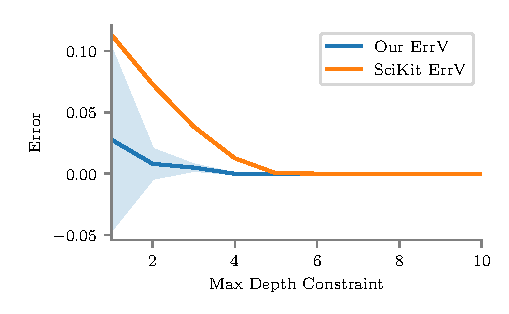
\includegraphics[width=\columnwidth]{figures/chart_ours_v_scikit_variance_mushrooms.pdf}
  \caption{Error ($\pm 2 \times \sigma$) for our algorithm versus scikit-learn on the \texttt{MUSHROOMS} dataset}
  \label{fig:mushoursvscikit}
\end{figure}

\begin{figure}
  \centering
  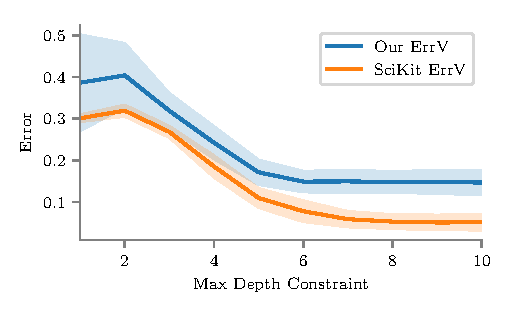
\includegraphics[width=\columnwidth]{figures/chart_ours_v_scikit_variance_tictactoe.pdf}
  \caption{Error ($\pm 2 \times \sigma$) for our algorithm versus scikit-learn on the \texttt{TICTACTOE} dataset}
  \label{fig:tttoursvscikit}
\end{figure}

The \texttt{CARS} dataset proved the most interesting. While our algorithm had worse accuracy than scikit-learn for small depth values, as the allowed depth increased we began to outperform scikit-learn's algorithm (figure \ref{fig:caroursvscikit}).

\begin{figure}
  \centering
  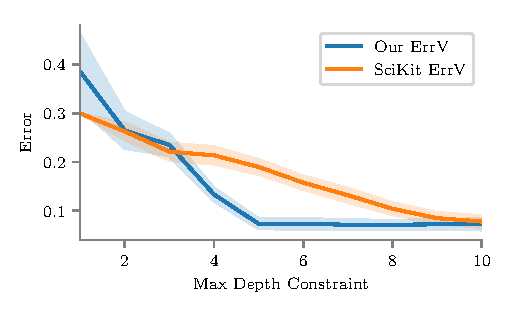
\includegraphics[width=\columnwidth]{figures/chart_ours_v_scikit_variance_car.pdf}
  \caption{Error ($\pm 2 \times \sigma$) for our algorithm versus scikit-learn on the \texttt{CARS} dataset}
  \label{fig:caroursvscikit}
\end{figure}

Overall, we found that our algorithm performed much worse on datasets with a large amount of interconnected data, such as Tic-Tac-Toe, where the impact of one attribute was heavily dependent on all of the other attributes. However, for more traditional classification problems, such as evaluating cars or mushrooms, our algorithm was very accurate.

\section{Discussion}

We were surprised at the discrepancies between our algorithm and the one provided by scikit-learn, as we expected both decision tree algorithms to produce similar results. While an effort was made to produce similar constraints on both algorithms (scikit-learn was used with the ``entropy'' heuristic, as well as the same tree depth constraint), there were a few differences that we were unable to resolve. First, scikit-learn uses ``an optimised version of the CART \cite{DBLP:books/wa/BreimanFOS84} algorithm.''

Additionally, scikit-learn cannot be used with categorical data. To get around this restriction, we used one-hot encoding for the scikit-learn algorithm. This has a negative impact on the depth: scikit-learn's decision tree is forced to be a binary tree, and so depth constraints act far more harshly than they do on our algorithm.

\section{Role Assignment \& Contributions}

\subsection{Alic}

Alic was responsible for implementing the decision tree learning algorithm, the JSON decision tree representation, helped improve the binary executables, and implemented unit testing for several core functions. He implemented the decision tree learning algorithm from Russell and Norvig \cite{russell_norvig_2010}, and added an optional depth constraint. He also was responsible for constructing both the internal decision tree representation and determining the JSON representation for communicating between the \texttt{dtl} and \texttt{classify} binaries. Additionally, he improved the binary executable command-line experience, enabling order-independent options as well as a \texttt{--help} option. Finally, he wrote unit tests for core functions such as \texttt{Plurality-Value}, \texttt{Entropy}, and \texttt{DecisionTreeLearning} itself. He was the project checker.

\subsection{Willem}

Willem worked primarily on decision tree creation, data file read in, and model selection in ocaml. He created a data reader for CSV files, which was used by all of the OCaml binaries (\texttt{dtl}, \texttt{classifier}, and the OCaml-based model selection program). He helped program the \texttt{dtl} executable, which reads in a data file for the training data, then creates a decision tree. He also wrote up the large amount of hard coded information about the different sets of data, including information about the attributes, their possible values, the possible classification, etc. He also created the OCaml version of model selection using cross validation, which takes in various optional and required command line arguments and prints out the selected tree, error rate in the training set, error rate in the validation set, and the chosen max depth. He also elected to be the project recorder.

\subsection{Diego}

%% The acknowledgments section is defined using the "acks" environment
%% (and NOT an unnumbered section). This ensures the proper
%% identification of the section in the article metadata, and the
%% consistent spelling of the heading.
\begin{acks}
This work was supported in part by the University of Iowa.
\end{acks}

\bibliographystyle{ACM-Reference-Format}
\bibliography{tech-report}

\appendix

\section{Supplemental Graphs \& Data}

\begin{figure}[h]
  \centering
  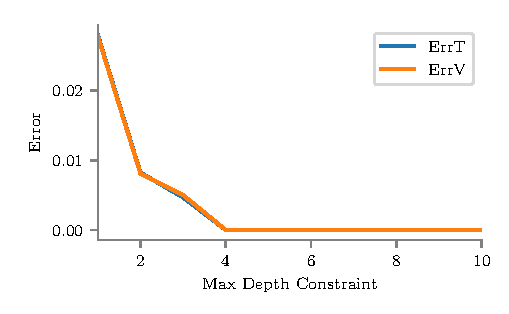
\includegraphics[width=\columnwidth]{figures/chart_errt_errv_mushrooms_ours.pdf}
  \caption{The error on training and validation data for the \texttt{MUSHROOMS} data set}
  \label{fig:mushroomserrterrv}
\end{figure}

\begin{figure}[h]
  \centering
  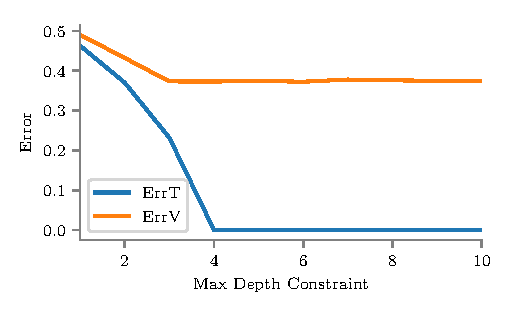
\includegraphics[width=\columnwidth]{figures/chart_errt_errv_balance_ours.pdf}
  \caption{The error on training and validation data for the \texttt{BALANCE} data set}
  \label{fig:mushroomserrterrv}
\end{figure}

\begin{figure}[h]
  \centering
  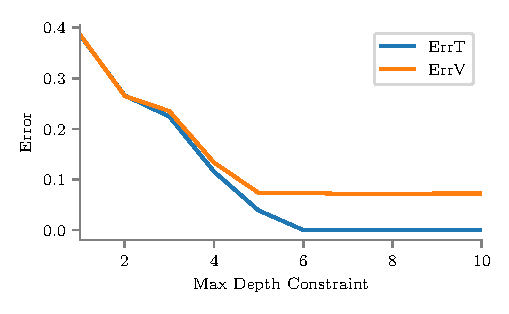
\includegraphics[width=\columnwidth]{figures/chart_errt_errv_car_ours.pdf}
  \caption{The error on training and validation data for the \texttt{CARS} data set}
  \label{fig:mushroomserrterrv}
\end{figure}

\begin{figure}[h]
  \centering
  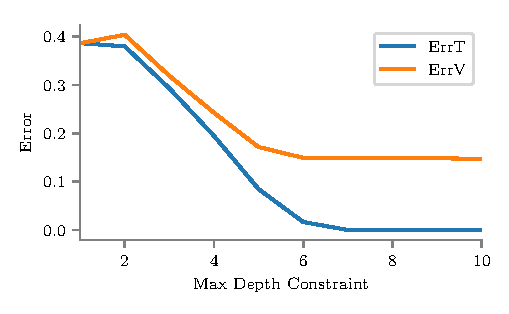
\includegraphics[width=\columnwidth]{figures/chart_errt_errv_tictactoe_ours.pdf}
  \caption{The error on training and validation data for the \texttt{TICTACTOE} data set}
  \label{fig:mushroomserrterrv}
\end{figure}

\end{document}
\endinput